\chapter{Détection d'objets et apprentissage profond}
\newpage
\pagestyle{fancy}
\fancyhead[L]{\chaptername \ \thechapter}
\fancyhead[R]{Détection d'objets et apprentissage profond}
\renewcommand{\headrulewidth}{1pt}
\fancyfoot[C]{\thepage}
\section{Introduction} 
Au début de l'intelligence artificielle avec la limitation des ressources de calcul, les chercheurs ou les programmeurs devaient choisir et extraire manuellement les caractéristiques, puis appliquer un algorithme tel que la régression ou la classification en fonction des caractéristiques extraites. Cela a limité les performances des modèles et ses résultats en raison des capacités limitées d'un humain à extraire les bonnes caractéristiques, en particulier lorsque les données contiennent une grande quantité de caractéristiques à extraire, ce qui affecte considérablement les performances des modèles.

Avec l'augmentation drastique de la puissance de calcul du matériel moderne, cela a permis d'implémenter un nouvel algorithme qui a résolu le problème précédent d'extraction de caractéristiques et a également créé un nouveau domaine d'intelligence artificielle qui est l'apprentissage en profondeur.

L'apprentissage en profondeur est basé sur des réseaux de neurones avec de nombreuses couches cachées qui, à leur tour, effectuent l'extraction de caractéristiques avec l'objectif du modèle (comme la classification). La première couche du réseau de neurones qui est la couche d'entrée (certains ne l'appellent pas une couche car elle ne contient aucun neurone). Cette couche transmet les données à la couche suivante où résident réellement des neurones, chaque neurone reçoit 1 ou plusieurs entrées de la couche précédente, puis applique un algorithme de calcul tel que : Régression linéaire \(Z = W * X + b\) où w est le poids ou Convolution : \(Z = X * f\) où les valeurs X du noyau sont les poids du neurone. Après avoir calculé Z, la valeur est transmise à une fonction d'activation spécifique telle que : \(ReLu(x) = max(0,x)\) puis la valeur finale est transmise en tant qu'entrée pour la couche suivante jusqu'à ce qu'elle atteigne la couche finale qui produit la prédiction du modèle. Ces étapes sont appelées propagation vers l'avant là où le modèle prédit. 

D'autre part, la rétroporpagation où le modèle apprend, il fait que l'erreur après avoir calculé en comparant les sorties souhaitées aux sorties du modèle prédites, puis en la propageant aux couches précédentes où, pour chaque neurone, les poids sont ajustés en fonction de l'algorithme d'optimisation choisi comme : Gradient Descent.
\begin{figure}[H]
     \centering
     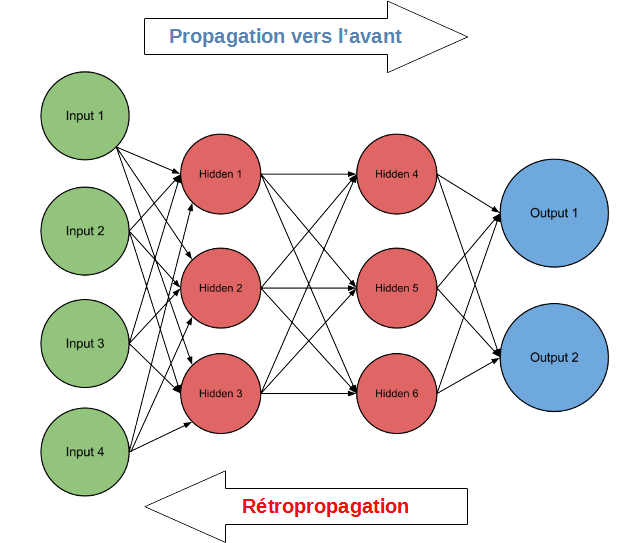
\includegraphics[height=12cm,width=12cm]{Chapitre2/img1.png}
     \caption{Structure d'un réseaux de neurones.}
     \label{img1}
     \end{figure}

\section{Concepts de base} 
% =========== CNN =========== 
     \subsection{Les réseaux de neurones convolutifs (CNN)} 
     De nombreux types de réseaux de neurones sont apparus pour résoudre des problèmes spécifiques, l'un d'eux est le réseau de neurones convolutifs (CNN), un réseau de neurones bien adapté pour traiter des tâches liées à la vision comme la reconnaissance d'objets. Ils ont été introduits pour la première fois en 1989, mais avec l'augmentation des pouvoirs de calcul et les grands ensembles de données d'imagerie, ils sont devenus le type de réseau neuronal de pointe pour la vision numérique.
     
     La structure CNN est inspirée du cortex visuel chez les animaux, où des groupes de cellules sont sensibles à une petite sous-région de l'image d'entrée. Par conséquent, l'image n'est pas traitée comme un bloc unique mais comme une composition d'éléments plus petits. \cite{db3}
     
     Le réseau de neurones contient plusieurs types de couches, chacune ayant un objectif spécifique et les couches les plus importantes sont :
     
     % =========== Convolution Layer =========== 
     \subsubsection{Couche de convolution}   
     La couche de convolution est la pierre angulaire du CNN. Il porte la partie principale de la charge de calcul du réseau où il effectue un produit scalaire entre 2 matrices : la première est le noyau, un ensemble de poids apprenables qui sont également les caractéristiques extraites et la seconde matrice est un ensemble de valeurs contenues dans le glissement fenêtre sur l'image, glissant d'un pas donné.
     \begin{figure}[H]
          \centering
          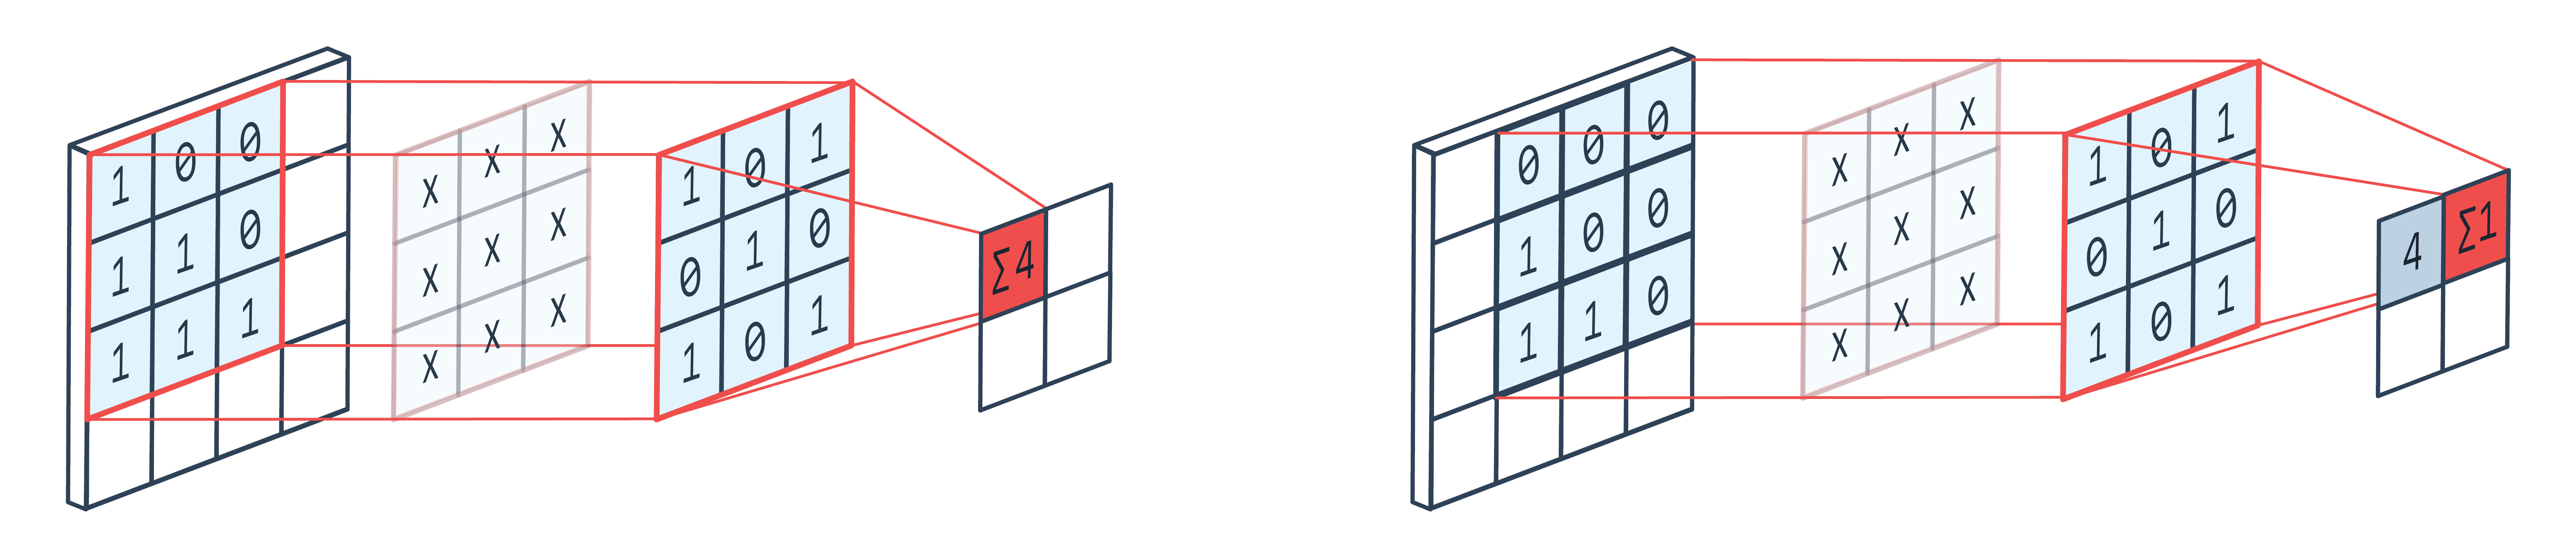
\includegraphics[height=5cm,width=15cm]{Chapitre2/img2.png}
          \caption{Structure de Couche de convolution. \cite{db4}}
          \label{img2}
          \end{figure}
     
     % =========== Pooling Layer ===========
     \subsubsection{Pooling Layer}   
     Ou sous-échantillonnage, Il sert généralement de médiateur entre plusieurs couches de convolution. Max-pooling et Average-pooling sont les stratégies de mise en commun les plus fréquemment utilisées dans les CNN. La mise en commun apporte de nombreux avantages aux CNN. En particulier, la mise en commun vise à empêcher le surajustement en concentrant les données locales avec une fenêtre de mise en commun réduisant ainsi la dimensionnalité des données. La réduction de la dimensionnalité des données permet également de réduire les calculs.
     \begin{figure}[H]
          \centering
          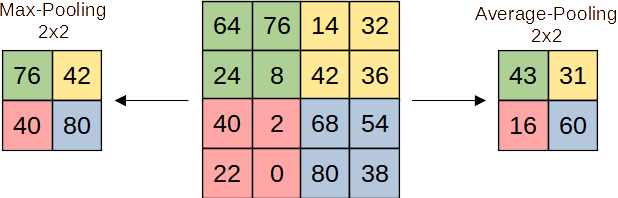
\includegraphics[height=5cm,width=15cm]{Chapitre2/img3.png}
          \caption{Max-pooling et Average-pooling.}
          \label{img3}
          \end{figure}
     
     % =========== Fully Connected Layer ===========
     \subsubsection{Fully Connected Layer (FC)}   
     Cette couche prend la sortie de convolution/polling, l'aplatit et prédit la meilleure étiquette pour décrire l'image. Comme dans un réseau neuronal à anticipation normal, les entrées de la couche entièrement connectée sont multipliées par les poids et additionnées. Ensuite, une fonction d'activation est utilisée pour produire la sortie comme Softmax qui est largement utilisée dans les problèmes de classification.
     \begin{figure}[H]
          \centering
          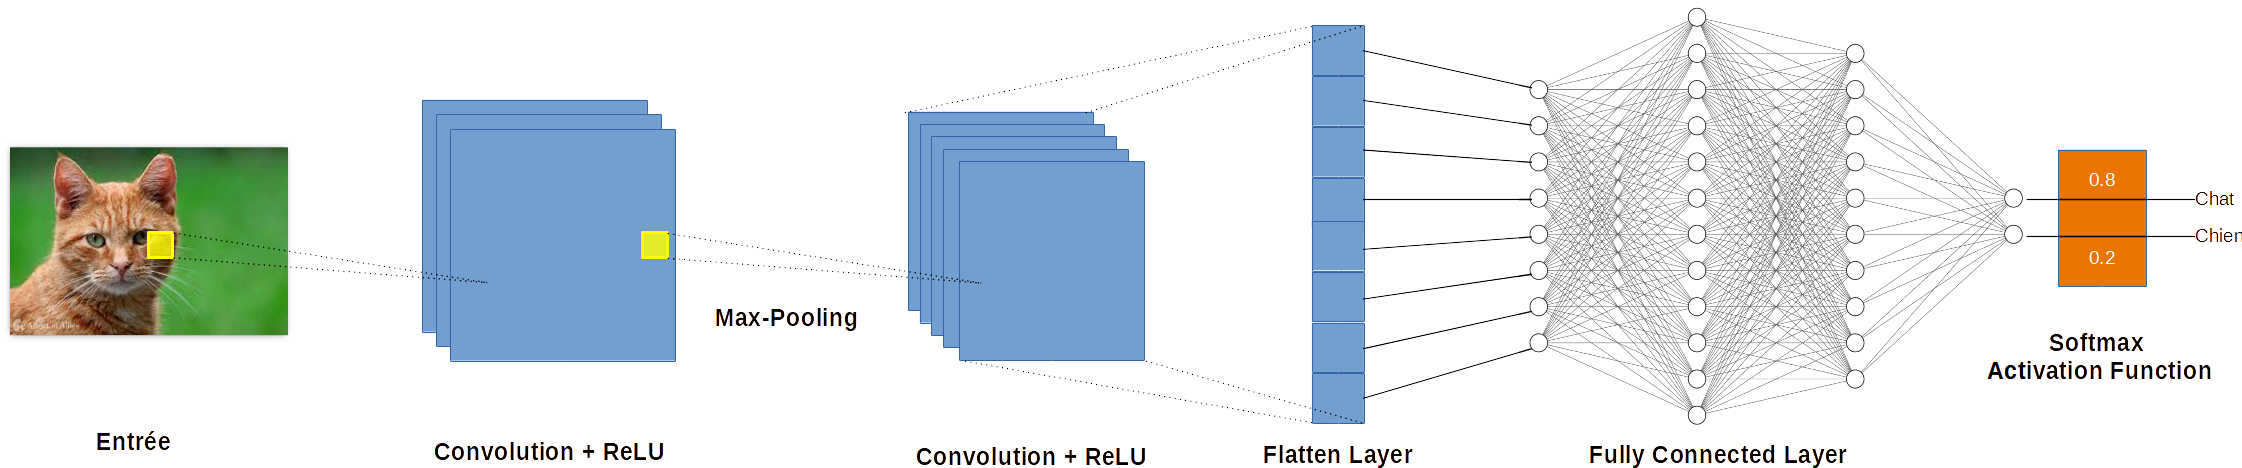
\includegraphics[height=4cm,width=18cm]{Chapitre2/img4.png}
          \caption{Exemple de structure de réseaux de neurones convolutionnels.}
          \label{img4}
          \end{figure}

% =========== Transfer Learning ===========
     \subsection{L'apprentissage par transfert} 
     L'apprentissage par transfert se produit lorsque des modèles existants sont réutilisés pour résoudre un nouveau défi ou problème. L'apprentissage par transfert n'est pas un type distinct d'algorithme d'apprentissage automatique, mais plutôt une technique ou une méthode utilisée lors de la formation de modèles. Les connaissances acquises lors des formations précédentes sont recyclées pour aider à effectuer une nouvelle tâche. La nouvelle tâche sera liée d'une certaine manière à la tâche précédemment formée.

     Le processus prend des parties pertinentes d'un modèle existant et les applique pour résoudre un problème nouveau mais similaire. Un élément clé de l'apprentissage par transfert est la généralisation. Cela signifie que seules les connaissances pouvant être utilisées par un autre modèle dans différents scénarios ou conditions sont transférées. Au lieu que les modèles soient liés de manière rigide à un ensemble de données de formation, les modèles utilisés dans l'apprentissage par transfert seront plus généralisés. Les modèles développés de cette manière peuvent être utilisés dans des conditions changeantes et avec différents ensembles de données.
     \begin{figure}[H]
          \centering
          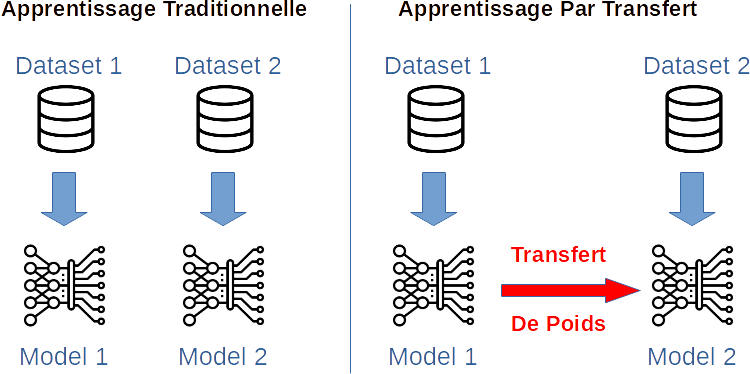
\includegraphics[height=7cm,width=13cm]{Chapitre2/img5.png}
          \caption{Différence entre l'apprentissage traditionnel et l'apprentissage par transfert.}
          \label{img5}
          \end{figure}

\section{Les méthodes de détections d'objets basées sur l'apprentissage profond} 
% =========== Architectures CNN populaires =========== 
     \subsection{Architectures CNN proposées populaires} 

\section{Métriques pour l'évaluation des systèmes de détection d'objets} 

\section{Bases de données d'évaluation} 
Les bases de données d'évaluation jouent un rôle très crucial dans la recherche, ceux sont l'un des facteurs les plus importants pour les progrès dans le domaine, malheureusement les données sont plus difficiles et plus coûteuses à générer. Au cours de la dernière décennie, un certain nombre d'ensembles de données ont été rendus publics pour évaluer les algorithmes de détection d'objets. Ces ensembles de données sont collectés à partir de différents scénarios et peuvent donc être utilisés comme référence pour les applications. Ci-dessous, nous décrivons les ensembles de données  les plus populaires utilisés pour l'évaluation dans ce domaine:

\begin{itemize}
\item Microsoft COCO \cite{db1}

\item ImageNet \cite{db2}
\item 
\item 
\item 
\end{itemize}



\section{Conclusion} 
